% !TEX root = ../main.tex
\chapter{帕金森疾病的智能辅助预测} 
\label{chapter:pdPrediction}
%帕金森病(PD)作为神经运动功能障碍及神经组织退行性变疾病中最为普遍和常见的一种,目前面临的主要挑战之一是许多患者在临床确诊时已经处于疾病的中晚期,导致错过了进行最佳临床治疗的黄金时期\cite{de2019prognosis,papagno2018cognitive}。因此,需寻找更快速、准确、和有效的筛查方法,以便在早期阶段诊断PD患者。这一挑战促使了对机器学习(ML)在PD分类预测中的研究,ML技术的发展为智能辅助诊断与健康测评提供了智能决策技术,有望解决特殊情况下的误诊或无法确诊的问题。
%在当前的研究趋势中,对于PD预测的关键问题之一是如何克服临床诊断的滞后性,使患者能够更早地接受有效的治疗。多模态数据融合成为研究的热点之一,通过整合临床数据、基因表达数据和影像数据等不同类型的信息,有望提供更全面和准确的PD分类预测。

%在第\ref{chapter5.1:pdPredictReview}节中基于机器学习的智能辅助PD分类预测进行了综述,突出了机器学习技术在提高PD智能辅助诊断与健康测评方面的潜力。ML模型的发展不仅有助于解决特殊情况下的误诊或无法确诊的问题,而且通过挖掘海量数据中的潜在规律,构建了一套相应规律的决策模型,为早期诊断提供了新的可能性。
%在第\ref{chapter5.2:pdCMF-Net}节中,我们提出了一种跨模态数据融合的机器学习方法(CMFP),通过综合利用基线DTI和临床特征数据,提出了一种智能辅助PD进展预测的创新方法。该方法的重要性在于通过纵向数据研究方法,结合机器学习,建立了早期PD基线DTI及临床特征的疾病进展模型。研究结果表明,跨模态的数据融合能够显著提高单模态预测的精确度,尤其在传统机器学习方法的应用中。这一发现为未来的PD研究提供了新的思路,强调了跨模态数据融合在提高预测性能方面的潜在优势。

PD的发生机制因素除复杂性外,还涵盖了遗传背景、环境暴露及生活习惯等多个层次的交织影响。其中,$\alpha$-突触核蛋白聚合现象是其生物学标识的核心组成部分。现有多模态影像整合技术在探究医学信息与影像特征深层次相关性方面存在不充分的问题,这在一定程度上限制了其在脑部疾病诊断中的表现力。
为了提升对PD等多种脑疾病的精确诊断能力,亟需引入跨模态数据集成分析的方法。
机器学习(ML)技术的进步为智能辅助诊断与健康评估提供了智能的决策支持,有望应对特殊情况下的误诊或难以确诊的挑战。第\ref{chapter5.1:pdPredictReview}节综述了ML的智能辅助PD分类预测方法\cite{jyWen}。ML模型通过挖掘大量数据中的隐藏规律,为早期辅助诊断提供了新的机会。
在第\ref{chapter5.2:pdCMF-Net}节中,提出了一种跨模态数据融合的ML方法(CMFP),它是通过综合DTI和临床数据的一种PD早期进展预测的新方法,可显著提高单模态预测的精确度。

\section{引言}
%帕金森病(PD)是一种以神经运动功能障碍和神经组织退行性变为特征的常见疾病。目前,我们面临的一个主要问题是,许多患者在确诊时已经进入疾病的中晚期,从而错过了最佳的治疗时机\cite{de2019prognosis,papagno2018cognitive}。为了解决这个问题,我们需要寻找更快速、更准确、更有效的筛查方法,以便能够及早地诊断出PD患者。这样做可以帮助我们更早地开始治疗,从而可能改善患者的预后和生活质量。

PD 是一种常见的神经系统疾病,主要影响人类的神经系统和运动控制\cite{2020Comparison},表现为静止时的颤抖、动作缓慢、身体活动受限以及平衡失调\cite{ameiPhdthesis}。PD随时间缓慢恶化,诊断依赖于患者的临床症状;肢体功能障碍和非运动症状不仅损害生活品质,还与较高死亡率相关,故早期预测和及时治疗至关重要\cite{agosta2015propagation}。至今为止,尚未发现能够准确反映PD的疾病进程的临床数据或生物指标\cite{ameiPhdthesis}。而且,对临床效果的评估往往需要较长的时间,且其结果易受到患者当时健康状况的影响而发生变化\cite{ameiPhdthesis}。标准的MRI能够展现清晰的组织差异,但在诊断疑似PD患者方面,它的主要价值在于帮助排除其他脑部疾病,而不是直接用来确认是否为PD\cite{post2008clinical}。PD 是一个异质性疾病,根据起病的年龄、临床表现及进展的快慢可以被分成不同的亚型\cite{thenganatt2014parkinson,rajput2009course}。PD疾病的发展会随着时间的演变而发生不同的变化,一些患者病情会保持稳定,而一些则进展为帕金森病痴呆(PDD)。因此,有必要预测PD疾病的进展。

研究发现,白质微观结构的变化在皮层神经元显著退化前就已发生,且这种变化未必与灰质体积减少相关\cite{ameiPhdthesis}。通过使用扩散张量成像(DTI)技术,研究者能够监测到帕金森病患者的大脑白质损伤,并发现这些损伤的程度与患者接下来一年中运动能力和认知功能的改变有着紧密的联系\cite{ameiPhdthesis,schwarz2013diffusion}。最新研究运用DTI技术揭示,在早期PD患者中,全脑体素分析指出胼胝体的分数各向异性(FA)和平均弥散度(MD)出现了明显的变化,特别是在膝部和压部区域更为显著\cite{amandola2022longitudinal}。研究还发现,胼胝体FA值的降低与大脑广泛皮质及皮质下区域的FA和MD值降低存在相关性\cite{amandola2022longitudinal}。进行多元回归分析后,结果表明在研究的起始点及两年后的跟进中,患者的运动刚性程度与胼胝体的FA值之间存在显著的负向关联,且这种关联在胼胝体前部区域最为突出。这些发现提示研究者们,在PD的早期阶段,胼胝体的微观结构变异可能是一个有用的生物标志物,用于监测运动刚性症状及其疾病进程的变化\cite{amandola2022longitudinal}。

\begin{table}[htbp]
\centering
\caption{基于机器学习技术在PD某一时刻智能辅助预测的相关工作}
\label{paper4MLpredictJt}
\small
\begin{tabular}{p{1.8cm}<{\centering}p{3.2cm}<{\centering}p{3.4cm}<{\centering}p{1.35cm}<{\centering}p{1.35cm}<{\centering}}
%\begin{tabular}{cccccc}
\hline 
\multicolumn{1}{c}{文献}  &方法    &数据及来源 &ACC(\%) &AUC(\%)  \\ \hline
文献\cite{sivaranjini2020deep}    &Transfer Learning (AlexNet)  &PMI 中的 MRI  &88.90  & -  \\ \\
文献\cite{martinez2018convolutional}   &Lenet 和Alexnet  &PPMI 中的 FP-CIT SPECT  &94.10  &98.40   \\ \\
文献\cite{kim2018artificial}    &Transfer Learning (Inception V3)  &PPMI 中的 SPECT  & -  &87.00   \\ \\
文献\cite{castillo2018robust}    &SVM和KNN的集成分类  &PPMI 中的 SPECT 和多种异质生物标志物
(CSF,Plasma,RNA和 Serum)  &96.00  & -   \\ \\
文献\cite{al2021feature}    &RF、XGBT和CatBoost的集成分类  &UCI 库中的声学特征  &86.25  & -   \\ \\
文献\cite{almeida2019detecting}   &KNN,MLP,OPF 和 SVM  &文献\cite{vaiciukynas2017detecting}中的发音与语言数据  &94.55  &87.00   \\ \\
文献\cite{nahar2021feature}    &GBT,XGBT,Bagging 和ExtraTree  &UCI 库中的声学特征  &82.35  & -   \\ \\
文献\cite{patra2019prediction}    &DT,LR和KNN的集成分类  &UCI 库中的声学特征  &84.59  & -   \\ \\
文献\cite{wang2020early}  &文献\cite{wang2020early}中提出的一种新颖的深度
学习方法  &PPMI中的REM,CSF、嗅觉丧失和SPECT数
据  &96.45  & -   \\ \\
文献\cite{prashanth2016high}     &NB,SVM,Boosting 和RF  &PPMI 中的睡眠行为障碍、CSF、嗅觉丧失和
DAT 数据  &96.40  &98.88   \\ \\
文献\cite{grover2018predicting}   &DNN  &UCI 库中的声学特征  &81.67  & -   \\  \\
文献\cite{masud2021crowd}   &文献\cite{masud2021crowd}中提出的一种新颖的深度
学习方法(CROWD)  &UCI 库中的声学特征  &96.00  & -   \\ \\
文献\cite{pahuja2022deep}    &CNN  &PPMI 中的 MRI,SPECT 和CSF  &93.33  & -   \\  \hline

\end{tabular}
\end{table}

%帕金森病是一种慢性退行性疾病,主要影响人类的神经系统和运动控制\cite{2020Comparison}。虽然PD的主要症状是运动障碍,如僵硬,但随着PD的进展,极有可能出现非运动症状,如抑郁或认知障碍\cite{2020Development}。随着人口老龄化的增加,帕金森病患者也在迅速增加,因此,用于评估和跟踪帕金森病的远程监测和远程诊断设备的进展已变得越来越重要\cite{2020Optimized,2005Fluorodopa}。Raval等人开发了一个模型,使用步态和姿势稳定性的临床测量和生物力学测量来预测个人PD超过两年的进展,该研究也证明了通过机器学习分析临床和生物力学测量来预测个体PD进展率和丰富试验的潜力\cite{2019Prediction}。Nguyen等人的工作中,来自82名帕金森病受试者的ReHo和fALFF特征被用于训练机器学习预测基线临床严重程度和进展,随访1年、2年和4年,这是第一次将rs-fMRI和机器学习结合起来预测未来的疾病进展\cite{2020Predicting}。在临床上,预测轻度认知障碍(MCI)的进展和诊断帕金森病(PD)的痴呆是困难的。Yang等人专注于研究帕金森病进展过程中脑结构连通性的改变,通过连接组范围的关联分析来检测随着PD进展的脑结构网络的重组,研究表明大脑皮层和皮层下的8个脑种子区随着PD的进展表现出显著的结构模式变化\cite{2021Alteration}。当前只有较少的学者研究全DTI和临床特征的结合预测PD进展,但其对PD的进展至关重要。DTI数据具有异质性,可描述早期PD疾病微观白质的变化。Shu等人开发和验证了基于全脑白质和临床特征的放射组学模型,以预测帕金森病(PD)的进展,也说明了传统结构MRI可以预测PD的进展\cite{2020Predicting2}。

ML,特别是与数据挖掘技术相结合时,关注的是一种算法的发展,它可以从已知数据中学习规律形成模型,然后将模型应用到未知数据中进行预测\cite{kuang2015comparison}。因此,ML被广泛应用于PD及其进展的预测,以提高其预测\cite{hill2017parkinson,2018A,2020Machine}的性能。目前的统计模型预测PD的临床进展具有挑战性。过去来自横断面试验的单变量纵向或多变量分析在预测单个结果或单个时刻的能力有限\cite{2017Predicting}。因此,跨模态及混合模型的设计将有利于PD进展的研究。

\section{基于机器学习的智能辅助预测技术}\label{chapter5.1:pdPredictReview}

\begin{table}[htbp]
\centering
\caption{基于机器学习在PD智能辅助进展预测的相关工作}
\label{paper4MLpredictDt}
\small
\begin{tabular}{p{1.8cm}<{\centering}p{3.2cm}<{\centering}p{3.4cm}<{\centering}p{1.35cm}<{\centering}p{1.35cm}<{\centering}}
%\begin{tabular}{cccccc}
\hline
\multicolumn{1}{c}{文献} &方法    &数据及来源 &ACC(\%) &AUC(\%)  \\ \hline
文献\cite{latourelle2017large}    &BN  &PPMI 中的临床、分子和基因数据  & -  & -   \\ \\
文献\cite{simuni2016predictors}    &RF  &PPMI 中的受试者人口统计学、疾病特征、
CSF 和DAT 数据  & -  & -   \\ \\
文献\cite{nilashi2020remote}   &DBN,SVR和 SOM  &基于真实世界 PD 数据的 Total-UPDRS 和
Motor-UPDRS  & -  & -   \\ \\
文献\cite{bi2021novel}    &CERNNE  &PPMI 和 ADNI 中的 SNP 和 fMRI  &88.60  & -   \\ \\
文献\cite{lei2017joint}    &SVM  &PPMI中的临床评分(睡眠、嗅觉)、MRI和DTI  &92.08  &94.44   \\ \\
文献\cite{kiryu2019deep}    &CNN  &英国脑库中的 MRI  &96.80  &99.50   \\ \\
文献\cite{adams2021improved}    &CNN  &PPMI 中的 DAT,SPECT 和非成像临床指标
(UPDRS\_III 评分)  &83.00  &90.00   \\ \\
文献\cite{khoury2019data}    &KNN,DT,RF,NB,SVM,
K-Means 和GMM  &PhysioNet 网站上的步态周期 vGRFs  &90.00  & -   \\ \\
文献\cite{khoury2018cdtw}    &KNN,DT,RF,SVM和GMM  &PhysioNet 网站上的步态周期CDTW  &97.00  & -   \\ \\
文献\cite{prince2018multi}   &多源集成学习与CNN  &mPower 数据集文献\cite{he2016deep}中的敲击、行走、声
音和记忆数据  &82.00  & -   \\  \hline
\end{tabular}
\end{table}

本节将PD的预测归纳为静态与动态(进展)预测\cite{jyWen}。静态预测方法通常依赖于某一特定时间点的临床基线数据来进行分类预测。这种方法只考虑了单一时刻的数据,而没有将随时间变化的数据纳入考量。多数相关研究采用这种方式来尝试预测疾病发展情况,如\cite{sivaranjini2020deep,martinez2018convolutional,kim2018artificial,castillo2018robust,al2021feature,almeida2019detecting,nahar2021feature,patra2019prediction,wang2020early,prashanth2016high,grover2018predicting,masud2021crowd,pahuja2022deep}。另外,动态指代涉及到在一段时间内收集的多个连续的临床状态数据,用以进行分类预测。这种动态预测方式通过分析患者在不同时间点的数据变化,来更好地预测疾病的进展情况,例如PD的发展趋势。这种方法比静态预测更能反映疾病随时间的演变过程,因而对于制定长期的治疗计划和管理策略尤为重要。如文献\cite{latourelle2017large,simuni2016predictors,nilashi2020remote,bi2021novel,lei2017joint,kiryu2019deep,adams2021improved,khoury2019data,khoury2018cdtw,prince2018multi}。

本节在PubMed检索平台通过搜索PD的静/动态预测并统计出了近33年(1990—2022年)相关研究成果,如图\ref{paper4JinDongTai}所示。图\ref{paper4JinDongTai}显示,在过去33年间,PD的预测研究主要集中在静态预测领域,且自2010年以来研究数量呈现持续上升趋势,至2022年已增长至648篇。尽管动态预测的相关成果较少,但自2016年起其增长速度显著加快。这些研究表明,借助智能辅助技术可以有效促进临床诊断和疾病治疗。动态预测在医疗健康领域的研究与实践正在逐步扩展,并日益受到重视。

    \begin{figure}[htbp]
      \centering
      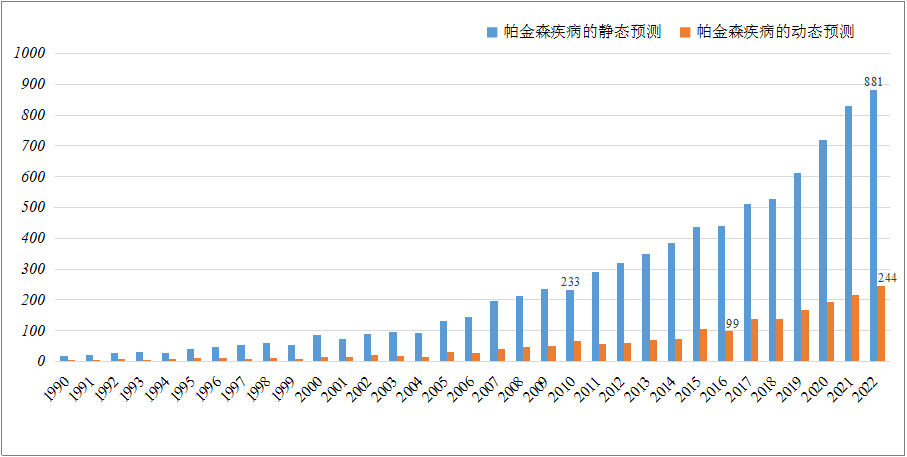
\includegraphics[width=0.9\linewidth]{figs/paper4JinDongTai.png}
      \caption{PD的静态及动态智能辅助预测发文量统计}\label{paper4JinDongTai}
     \end{figure} 

数据的丰富性提高、计算技术的进步以及神经网络设计的优化共同促进了深度学习技术的发展和普及。作为ML领域中的先进技术,深度学习通过构建更加复杂的神经网络来增强模型的表现力和准确度。在PD的预测领域,深度学习方法同样取得了令人瞩目的成效\cite{sivaranjini2020deep,prashanth2016high,vaiciukynas2017detecting,naranjo2016addressing,masud2021crowd,pahuja2022deep,sharanyaa2022optimized,oh2020deep,adams2021improved}。
表\ref{paper4MLpredictJt}和表\ref{paper4MLpredictDt}汇总了近年来运用机器学习技术对帕金森病(PD)进行静态和动态评估的多项研究成果,涵盖了所采用的不同ML技术、数据来源以及预测的准确率(ACC和AUC)。其中,大多数研究倾向于使用传统ML技术,而采用深度学习技术的研究相对少见。数据主要来自PPMI,并且大多数医学影像数据采用的是SPECT。在这些研究中,仅使用单一数据类型进行预测的成功率通常较低,而使用步态周期数据进行预测的成功率较高。同时,将脑脊液(CSF)等临床评分与医学影像数据相结合,能够显著提高预测的性能。


当前,多模态分类预测模型在帕金森病(PD)的研究中正逐渐受到重视并展现出发展潜力。尽管如此,这一领域仍面临诸多挑战,特别是在收集和整合PD患者全面数据方面存在限制。因此,开发无需人工干预即可从多种模态中自动提取特征的早期PD分类预测模型显得尤为重要。这样的模型能够利用更为丰富的数据资源,从而构建更精确的分类预测网络。此外,表\ref{paper4MLpredictDt}的分析表明,目前只有少数研究尝试结合基因数据与医学影像数据来探索它们与PD之间的关联。这种跨模态的数据融合方法有望进一步加深学者对PD遗传背景及其与疾病发展之间联系的理解。


\section{临床信息主导的智能辅助进展预测}\label{chapter5.2:pdCMF-Net}
随着人口老龄化的增加,帕金森病患者也在迅速增加,因此,对评估和跟踪帕金森病进展的动态监测变得越来越重要。为了找到一种更为高效的帕金森病进展预测方法,本节通过分析单模态(DTI、DAT及临床)特征在PD疾病5年后进展预测的临床价值,并提出一种跨模态数据融合(DIT\&临床、DAT\&临床)对帕金森病的进展进行预测的方法(Cross-Modal Fusion prediction model,CMFP)。
该方法的步骤主要是数据准备, 建模, 预测。数据涉及到临床, DTI及DAT这3种模态, 不同模态数据类型均使用Lasso方法进行特征筛选。各单模态采用AdaBoost进行分类, 将结果应用于新的融合策略CMF中得到新的模型。最后使用新的模型进行预测。CMFP在PD进展上的预测获得的AUC为0.7791。与单独的临床数据、DTI数据和DAT数据预测所获得的AUC分别提高了0.2448、0.3078、0.327。测试临床与DTI结合预测相对于单独使用临床数据预测的结果具有统计学显著性, p值为9.183e-4。该方法还确定了与PD相关的关键的脑区和重要的临床指标。本节的研究结果表明, CMFP是有效的, 其有助于改善单模态数据预测性能低的不足, 提高PD进展预测的准确性。并能确定PD的潜在生物标志物信息, 为了解PD提供了新的途径, 值得进一步研究。

\subsection{智能辅助预测的数据与方案}

    \begin{figure*}[ht]
      \centering
      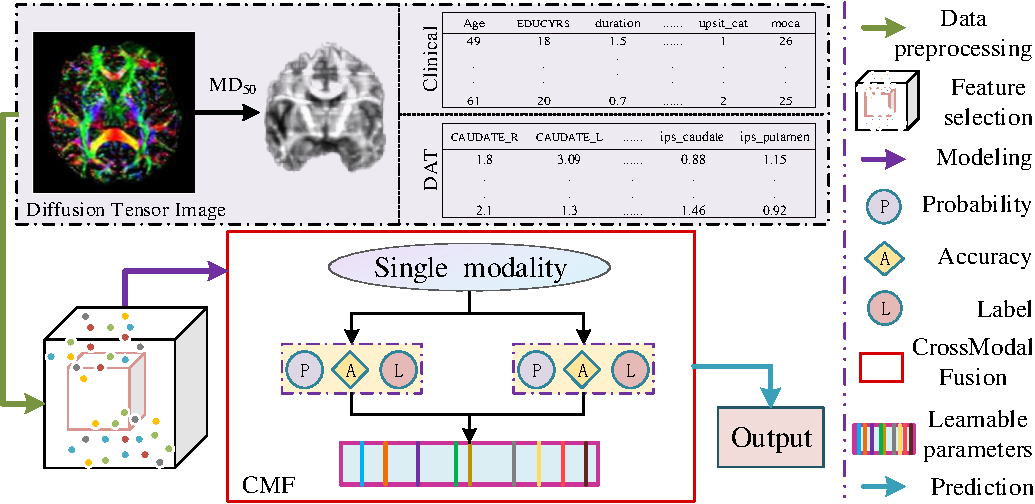
\includegraphics[width=0.9\linewidth]{figs/paper5FrameworkNew.pdf}
      \caption{本节提出的方法(CMFP)框架图}\label{paper5FrameworkNew}
     \end{figure*} 

\subsubsection{进展预测的数据说明}
本项研究利用了帕金森病进展标志物倡议(PPMI)的丰富资源,该资源汇集了多个研究中心的PD患者纵向数据。所有参与PPMI的研究站点均已获得相应伦理审批,且所有参与者在加入前都签署了知情同意书。研究中,本节采用HYS量表会考虑运动功能的退化、生活质量的降低以及多巴胺水平的减少等多个因素,并据此将PD分为五个不同的阶段(1至5期)。研究入选标准包括:至少有5年的纵向随访记录且HYS评分完整的PD患者;基线数据中含有完整的MRI影像资料,包括3D T1WI和DTI扫描;使用3T Siemens MRI进行扫描。筛选条件包括临床信息不完整、成像质量不佳以及图像处理出现失误等情况。

在本研究中,共有123名PD患者符合入选条件。通过分析PPMI数据库中这些患者5年的HYS评分动态,本节观察到74例患者的评分高于初始水平,46例患者评分持平,而3例患者评分低于起始水平。据此,本节将评分提升的患者定义为进展组(共72例),评分未变或下降的患者则归为稳定组(共49例)。研究还收集了一系列临床信息,包括性别、年龄、教育背景以及PD运动评定量表等,并测量了脑脊液中的生物标志物:A$\beta$42、$\alpha-syn$、$t-tau$和$p-tau$的蛋白浓度。123位受试者接受了3T Siemens MRI的非对比增强3D T1加权成像和DTI扫描。DTI影像的预处理使用了PANDA软件,包括去除非脑组织、纠正涡流效应和轻微头部移动、计算DTI矩阵以及应用连续跟踪(FACT)算法进行纤维追踪。若追踪过程中遇到曲率角度大于45°或体素分数各向异性(FA)值小于0.2,则追踪终止。在构ML模型时,本节选取了与PD进展相关的基线期临床指标、DAT水平及DTI脑网络特征作为输入变量,并运用Lasso的方法进行特征选择,旨在提升模型的预测准确度和泛化能力。


\subsubsection{进展预测的特征选择} 
在构建人工智能机器学习模型时,特征选择扮演着至关重要的角色,其重要性不容忽视。不同的特征选择会直接影响模型的预测准确性和在未见数据上的泛化能力。在本节的研究工作中,通过整合基线时的临床参数、多巴胺转运体(DAT)扫描数据以及扩散张量成像(DTI)所揭示的网络特性,本节创建了一个机器学习框架,用以预测五年后PD患者疾病的演变情况。为了提高模型的预测效果,本节对数据进行了严格的预处理,剔除了无效、不规范和错误的数据。
在原始的临床数据中,在本研究中,对16项临床指标进行了系统分析,这些指标包括三类基础信息、九种用于评估运动能力和认知水平的测试量表,以及四项反映脑脊液中蛋白质浓度的生化测量值。通过应用Lasso方法进行特征筛选,本节成功识别并保留了4个最为关键的临床变量(UPDRS Part III Score、UPDRS Total Score、Age、UPSIT score),这些变量与PD的疾病进展有着较高的相关性。对于DTI变量为脑区MD(50)矩阵,也使用Lasso方法进行数据选择,最终选择7个特征(Splenium of Corpus Callosum、Fornix (Column and Body of Fornix)、Inferior Cerebellar Peduncle (Left)、Superior Cerebellar Peduncle (Left)、Fornix (Crescent)/Stria Terminalis (Right)、Tapetum Left、Tapetum Right),分别代表终纹、胼胝体压部、穹窿、左侧小脑下脚、左侧小脑上脚、左内矢状层、右内矢状层这几个脑区。对于DAT数据,也使用Lasso方法进行数据选择,最终选择4个特征:
Putamen Left、High Putamen、Low Striatum和High Striatum,它们分别代表了左侧腹核、高腹核、低纹状体和高纹状体。这样的特征选择策略不仅提高了模型的解释能力,还有助于增强模型预测效果及应对不同情况的广泛适用性。



\subsubsection{跨模态数据融合的进展预测}
本节通过整合基线时的临床参数、多巴胺转运体(DAT)扫描数据以及扩散张量成像(DTI)所揭示的网络特性来训练机器学习模型,用以预测五年后PD患者疾病的演变情况。 在单模态建模过程中, 本节采用AdaBoost算法进行的分类。
AdaBoost(自适应增强算法)是一种集成方法,它能够将多个表现一般的弱分类器协同工作以构建一个强大的综合分类器。其“自适应”体现在:每当一个弱分类器在训练中对某些样本判断错误时,这些样本的权重会被相应增加。随后,在下一轮迭代中,所有样本根据更新后的权重再次参与训练新的弱分类器。此过程不断循环,每轮迭代都会依据全体样本调整权值并确定每个新加入的弱分类器的贡献度,继续迭代直到满足预定错误率条件或达到最大循环次数。AdaBoost能够根据弱分类器提供的信息动态调整错误率预期,并且以高效率运作,已有研究使用AdaBoost对PD进行早期预测\cite{anisha2020early}。

为了进一步改进单变量基线数据对5年后进展预测的性能, 本节采取跨模态数据组合的方式, 并提出一种新的决策策略以提高预测性能。图\ref{paper5FrameworkNew}是本研究的总框架图, 包括数据预处理, 特征筛选, 分类器建模, 预测4部分构成, 具体步骤:
%设置参数、数据准备、单模态训练、多模态融合、循环训练、模型保存、测试集验证
\begin{enumerate}
\item 设置参数epoch=120, 使用Adam作为优化算法, 初始学习率为0.01, 每50个epoch学习率下降0.1, 损失的计算采取的是MSE的计算过程, $\beta$为1 , $\alpha$为0.4;
\item 使用Lasso方法对多模态数据进行特征筛选, 将筛选出的特征作为训练集、验证集和测试集, 并按照6:3:1分配三个子集;%\item 3 分别单独输入两个不同模态的数据的训练集与验证集, 并打乱这两个集合的顺序;
\item 将不同的单模态的训练集数据使用AdaBoost方法进行训练, 得到的模型使用验证集数据进行预测, 得到预测的概率、预测的标签和精确度, 并分别保存单模态训练好的模型;
\item 将不同模态预测的结果(预测的概率、预测的标签和精确度)输入多模态融合算法(CMF:CrossModalFusion)中, 得到一组新的预测结果(预测的概率、预测的标签和精确度), 并保存融合模型;
\item 重复3-5步骤, 直到epoch=120结束循环;
\item 查找单模态训练过程中保存的精确度最高的模型Ms和两模态融合过程中保存的精确度最高的模型Mc。
\item 将测试集数据输入模型Ms, 得到预测的结果(预测的概率、预测的标签和精确度), 并将这组结果输入到模型Mc中进行测试, 得到两模态融合的预测概率和标签。
\end{enumerate}

在决策之前本节获取到了两种单模态数据的预测结果, 包括预测标签, 预测概率及精确度,分别记作$\rho_{a},~\rho_{b},~\eta_{a},~\eta_{b},~\varphi_{1}~and~\varphi_{2}$。根据这些单模态预测结果,使用本节提出的决策策略CMF可以得到决策融合的预测结果$\Phi$,它由预测概率和预测标签组成,即$\Phi = [\rho,~\eta].$。本节定义预测类别的差异$\Omega = abs(\rho_{a} - \rho_{b})$,即两个模型预测的类别之间的绝对差值。准确率的差异的符号$\sigma = sign(\varphi_{1} - \varphi_{2})$,即两个模型准确率之差的符号。sign函数返回-1、0或1,表示差异为负、零或正。预测概率的差异$\upsilon = abs(\eta_{a} - \eta_{b})$,即两个模型预测的概率之间的绝对差值。$\lambda$是通过概率差异$\upsilon$计算的权重。$\mathrm{\lambda=}\iota/(1+\mathrm{e}^{-\alpha * \upsilon} )$。其中,$\iota$为1 ,$\alpha$为0.4; 最终的预测概率和预测标签由公式(\ref{paper5pro})和(\ref{paper5pre})获得,根据$\Omega,~\sigma$和$\upsilon$的取值,选择不同的分支来组合预测结果。 $\zeta(A,~B,~C)$表示条件函数,如果$A$为真,则结果为$B$,否则为$C$。

\if 0
\begin{equation}\label{paper5Ldif}
\mathrm{\lambda=}\iota/(1+\mathrm{e}^{-\alpha * \upsilon} )
\end{equation}
\fi

\if 0
\begin{equation}\label{paper5proB}
\psi=\mathrm{\zeta}(\sigma>0,~\mathrm{\eta_{a}},~\mathrm{\eta_{b}})
\end{equation}

\begin{equation}\label{paper5proC}
\tau=\mathrm{\zeta}(\sigma>0,~\mathrm{\lambda}+\mathrm{\eta_{a}},~\mathrm{\lambda}+\mathrm{\eta_{b}})
\end{equation}

\begin{equation}\label{paper5pro}
\mathrm{\rho}=\mathrm{\zeta}(\Omega=0,~\psi,~\tau)
\end{equation}
\fi


\begin{equation}\label{paper5pro}
\mathrm{\rho}=\mathrm{\zeta}(\Omega=0,~\mathrm{\zeta}(\sigma>0,~\mathrm{\eta_{a}},~\mathrm{\eta_{b}}),~\mathrm{\zeta}(\sigma>0,~\mathrm{\lambda}+\mathrm{\eta_{a}},~\mathrm{\lambda}+\mathrm{\eta_{b}}))
\end{equation}



\if 0
\begin{equation}\label{paper5preB}
\phi=\mathrm{\zeta}(\sigma>0,~\mathrm{\rho_{a}},~\mathrm{\rho_{b}})
\end{equation}

\begin{equation}\label{paper5preC}
\mu=\mathrm{\zeta}(\mathrm{\rho}<0,~-1,~\mathrm{\rho}>0.5,~1,~0)
\end{equation}

\begin{equation}\label{paper5pre}
\mathrm{\eta}=\mathrm{\zeta}(\Omega=0,~\phi,~\mu)
\end{equation}
\fi

\begin{equation}\label{paper5pre}
\mathrm{\eta}=\mathrm{\zeta}(\Omega=0,~\mathrm{\zeta}(\sigma>0,~\mathrm{\rho_{a}},~\mathrm{\rho_{b}}),~\mathrm{\zeta}(\mathrm{\rho}<0,~-1,~\mathrm{\rho}>0.5,~1,~0))
\end{equation}



\subsection{智能辅助预测的实验分析}
本节使用的是Python 3.7.9语言编程,在GNU/Linux x86 64 system of GeForce RTX 3090 Ti 12 Intel Core Interl(R) Xeon(R) CPU E5-2678 v3 2.50GHz 64GB RAM 平台上运行。为了提高模型的性能,在输入模型进行训练与验证之前样本顺序都进行了随机的打乱。

\begin{table}[ht]
\centering
%\scriptsize
\caption{临床数据、DTI数据和DAT数据的特征组合 }
\label{paper5combinations}
%\begin{tabular}{c|ccccccc}
\begin{tabular}{p{1.5cm}<{\centering}|p{1.3cm}<{\centering}p{1.3cm}<{\centering}p{1.3cm}<{\centering}p{1.3cm}<{\centering}p{1.3cm}<{\centering}p{1.3cm}<{\centering}p{1.3cm}<{\centering}p{1.3cm}<{\centering}}
\hline  \hline
\textbf{$\delta_2$} & Age  & UP3s &      &      &           &     &     \\
\textbf{$\delta_3$} & Age  & UP3s & PTs  &      &           &     &     \\
\textbf{$\delta_4$} & Age  & UP3s & PTs  & Uts  &           &     &     \\
\textbf{$\delta_5$} & Age  & UP3s & PTs  & Uts  & STs       &     &     \\ \hline 
\textbf{$\gamma_2$} & SoCC & Fcb  &      &      & \textbf{} &     &     \\
\textbf{$\gamma_3$} & SoCC & Fcb  & ICPl &      & \textbf{} &     &     \\
\textbf{$\gamma_4$} & SoCC & Fcb  & ICPl & SCPl &           &     &     \\
\textbf{$\gamma_5$} & SoCC & Fcb  & ICPl & SCPl & FcSTr     &     &     \\
\textbf{$\gamma_6$} & SoCC & Fcb  & ICPl & SCPl & FcSTr     & TaR &     \\
\textbf{$\gamma_7$} & SoCC & Fcb  & ICPl & SCPl & FcSTr     & TaR & TaL \\ \hline 
\textbf{$\vartheta_2$}    & PuL  & HPu  &      &      &           &     &     \\
\textbf{$\vartheta_3$}    & PuL  & HPu  & LSt  &      &           &     &     \\
\textbf{$\vartheta_4$}    & PuL  & HPu  & LSt  & HSt  &           &     &    \\\hline \hline
\end{tabular}
\end{table}


\subsubsection{不同类型数据预测分析}
使用单一或双模态数据来预测帕金森病(PD)的进展会得到不同的结果。
表\ref{paper5singalAvg_AUC}展示了使用三种模态分别预测PD进展的平均AUC值,可以观察到每个AUC值相对较低。其中,$\Gamma$指的是特征选择,而$\Gamma_i$指代特定的特征组合,$i$表示组合的序号。不同数据集对应不同的特征组合,具体的特征组合显示在表\ref{paper5combinations}中。在表 \ref{paper5combinations}中,$\delta_{i}$,$\gamma_{i}$和$\vartheta_{i}$ 分别代表临床数据、DTI数据和DAT数据的特征组合,其中$i$表示特征组合的数量。$\Gamma_{21}$, $\Gamma_{23}$和$\Gamma_{50}$代表每个模态的所有特征组合。UP3s: UPDRS Part III score,PTs: UPDRS Total Score,Uts: UPSIT score,STs: STAI scores. SCC: Splenium of Corpus Callosum,Fcb: Fornix (Column and Body of Fornix),ICl: Inferior Cerebellar Peduncle (Left),SCl: Superior Cerebellar Peduncle (Left),FcSr: Fornix (Crescent)/Stria Terminalis (Right),TaR: Tapetum Right,TaL: Tapetum Left. PuL: Putamen Left,HPu: High Putamen,LSt: Low Striatum,HSt: High Striatum。


\begin{table*}[ht]
\centering
\caption{单模态数据预测PD进展的平均AUC值}
\label{paper5singalAvg_AUC}
\footnotesize
\begin{tabular}{cccccccccc}
\hline \hline
  & \textbf{$\Gamma_2$} & \textbf{$\Gamma_3$} & \textbf{$\Gamma_4$} & \textbf{$\Gamma_5$} & \textbf{$\Gamma_6$} & \textbf{$\Gamma_7$} & \textbf{$\Gamma_{21}$} & \textbf{$\Gamma_{23}$} & \textbf{$\Gamma_{50}$} \\ \hline
\textbf{Clinical}     & 0.4077      & 0.4371      & 0.4515      & 0.4478      & -           & -           & -            & 0.4629       & -            \\
\textbf{DTI}          & 0.4208      & 0.4476      & 0.4489      & 0.4310      & 0.4770      & 0.4191      & -            & -            & 0.4381       \\
\textbf{DAT}          & 0.5017      & 0.4767      & 0.4631      & -           & -           & -           & 0.4506       & -            & -      \\ \hline    \hline  
\end{tabular}
\end{table*}

   \begin{figure}[ht]
      \centering
      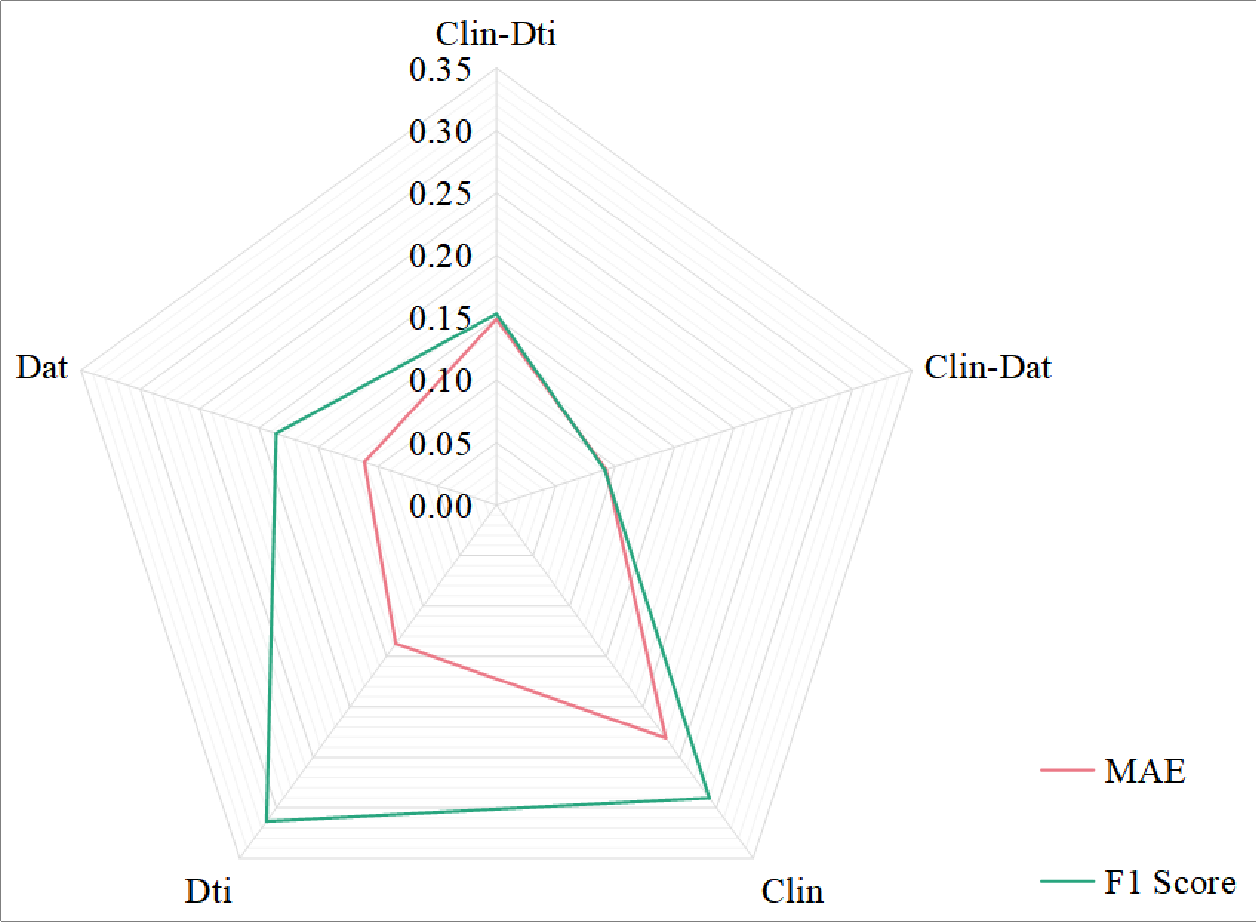
\includegraphics[width=0.85\linewidth]{figs/paper5MAEF1SCOREvariance.pdf}
      \caption{不同策略进行五次预测的MAE和F1 score的方差}\label{paper5MAEF1variance}
     \end{figure}

通过本节提出的跨模态融合预测方法(CMFP),对DTI和DAT的临床组合进行了测试,AUC结果如表\ref{paper5cmfDifferFeature_AUC}所示。其中,$\delta_i$,$\gamma_i$和 $\vartheta_i$分别代表临床数据、DTI数据和DAT数据的特征组合。它们的定义与表 \ref{paper5combinations} 中的相同。 表\ref{paper5cmfDifferFeature_AUC}中的A表示临床数据与DTI的结合预测;B表示临床数据与DAT的结合预测。不同数量的特征选择会导致AUC值的变化,当选择了4个临床特征和7个DTI特征时,结果相对较高,达到了0.7791。因此,在随后的分析中,将以该组合作为实验对象。然而,临床和DAT的联合预测效果相对较差。当选择2个临床特征和DAT特征进行预测时,AUC最高为0.6。使用本节提出的方法,对于预测4个临床特征和7个DTI特征的组合,方差为0.1085。相反,在预测2个临床特征和2个DAT特征的组合八次后,方差为0.1929。总体而言,临床和DTI的联合预测效果优于临床和DAT的联合预测效果。


    \begin{figure*}[ht]
      \centering
      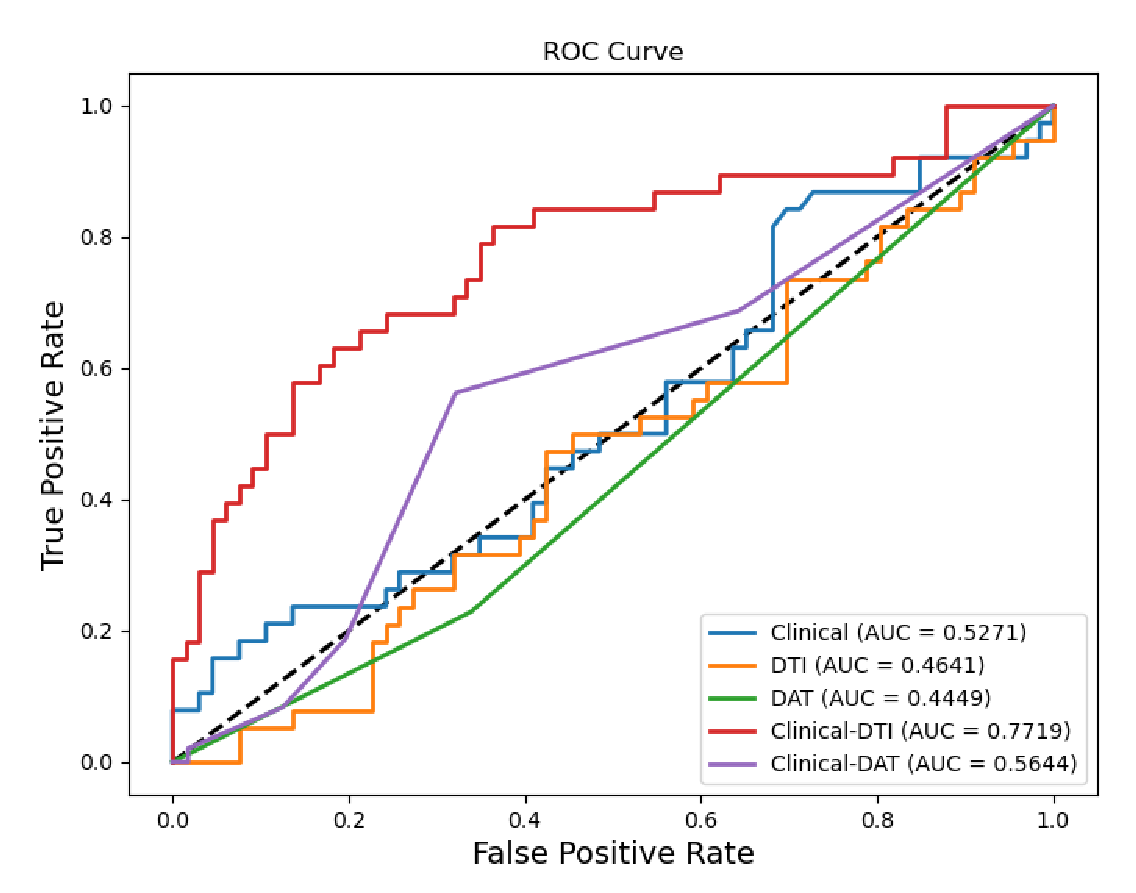
\includegraphics[width=0.95\linewidth]{figs/paper5ROCs_1case.pdf}
      \caption{五种不同策略预测PD进展的ROC曲线对比分析}\label{paper5ROCs_}
     \end{figure*}


在表 \ref{paper5cmfDifferFeature_AUC} 中可以观察到,当将临床数据的 4 个特征与 DTI 数据的 7 个特征结合起来进行预测时,所得到的 AUC 值在所有特征组合中表现最佳。同样地,当将临床数据的 2 个特征与 DAT 数据的 2 个特征结合起来进行预测时,也得到了更优异的 AUC 值。为了更深入地分析单模态数据预测和双模态数据预测的模型性能,计算了MAE和F1分数。图 \ref{paper5MAEF1}(a) 和 (b) 分别展示了五种预测情况的 MAE 和 F1 分数评估结果。其中,Clin-Dti代表临床数据与DTI结合的预测结果,Clin-Dat代表临床数据与DAT结合的预测结果。MAE 用于衡量预测结果与实际观察值之间的平均偏差。较小的 MAE 值表示模型的预测结果更接近真实值。而 F1 分数是基于精确度和召回率的调和平均值,较高的值表示模型的分类性能更好。

\begin{table}[htbp]
\centering
%\footnotesize
\caption{临床数据分别与DTI和DAT融合预测的AUC值}
\label{paper5cmfDifferFeature_AUC}
%\begin{tabular}{|c|ccccc|}
\begin{tabular}{|p{1.1cm}<{\centering}|p{1.8cm}<{\centering}p{1.8cm}<{\centering}p{1.8cm}<{\centering}p{1.8cm}<{\centering}p{1.8cm}<{\centering}|}
\hline
 \textit{\textbf{A}} & $\delta_{23}$         & $\delta_2$                   & $\delta_3$          & $\delta_4$                   & $\delta_5$          \\ \hline 
\textbf{$\gamma_{50}$}               &  0.6409   &  0.4647          &  0.5539  &  0.4873          &  0.4859  \\
\textbf{$\gamma_2$}                &  0.4955   &  0.5113          &  0.5506  &  0.5102          &  0.6459  \\
\textbf{$\gamma_3$}                &  0.5315   &  0.5161          &  0.5053  &  0.5193          &  0.5858  \\
\textbf{$\gamma_4$}                &  0.5458   &  0.4963          &  0.5435  &  0.4566          &  0.6038  \\
\textbf{$\gamma_5$}                &  0.5288   &  0.4936          &  0.4623  &  0.6019          &  0.4905  \\
\textbf{$\gamma_6$}                &  0.4872   &  0.6439          &  0.7096  &  0.5681          &  0.6135  \\
\textbf{$\gamma_7$}                &  0.6677   &  0.5228          &  0.4717  &  \textbf{0.7791} &  0.5172  \\ \hline
 \textit{\textbf{B}}  & $\delta_{23}$         & $\delta_2$                   & $\delta_3$          & $\delta_4$                   & $\delta_5$   \\ \hline 
\textbf{$\vartheta_{21}$}               &  0.5759   &  0.4670          &  0.4144  &  0.4606          &  0.4960  \\
\textbf{$\vartheta_2$}                &  0.5592   &  \textbf{0.6000} &  0.5683  &  0.5694          &  0.5842  \\
\textbf{$\vartheta_3$}                &  0.5591   &  0.5990          &  0.4982  &  0.4657          &  0.5146  \\
\textbf{$\vartheta_4$}                &  0.5729   &  0.5207          &  0.5518  &  0.5130          &  0.5882      \\
\hline 
\end{tabular}
\end{table}

   \begin{figure}[ht]
      \centering
      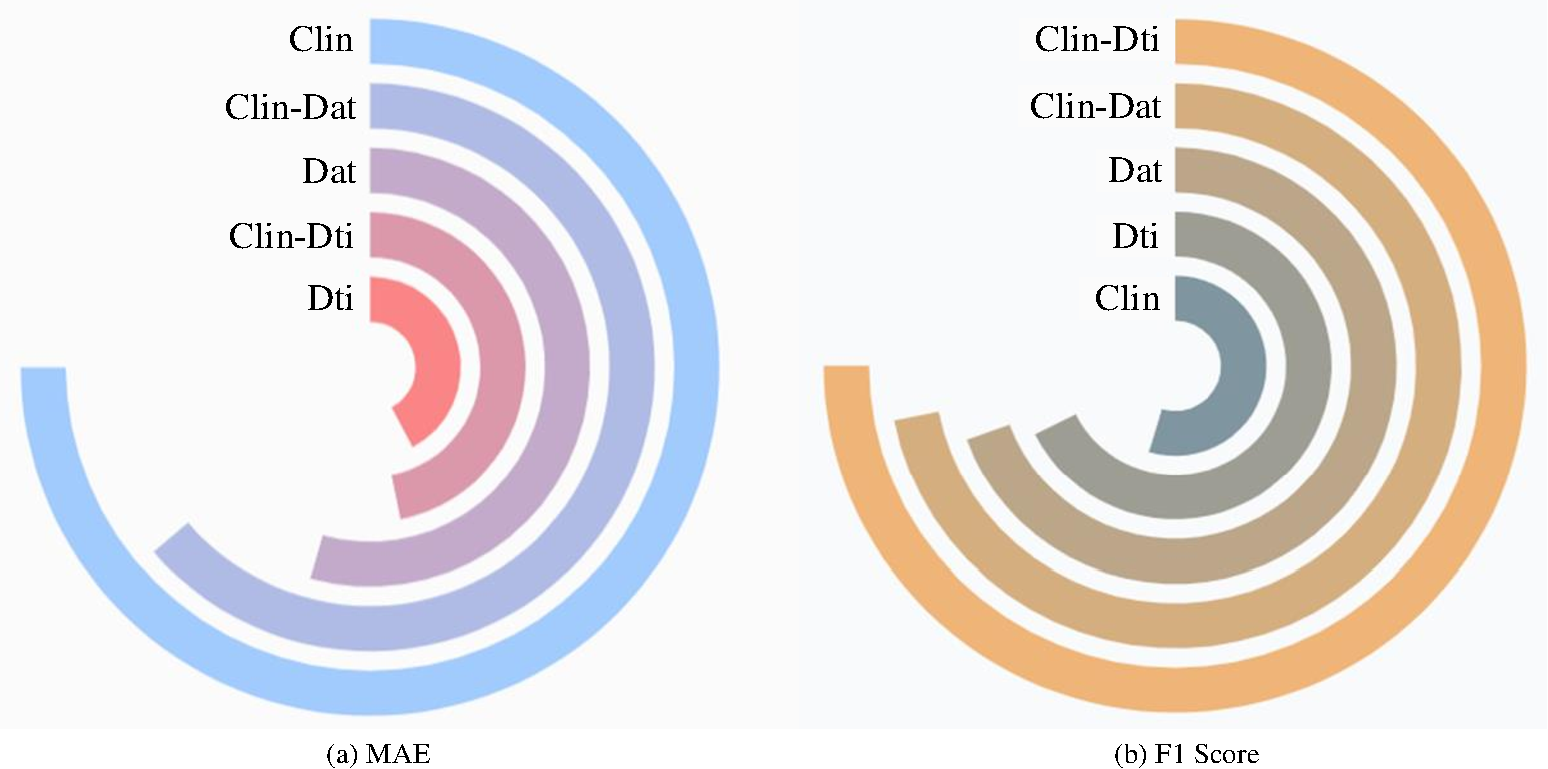
\includegraphics[width=0.95\linewidth]{figs/paper5MAEF1SCORE.pdf}
      \caption{采用不同策略进行五次预测PD进展的MAE和F1得分的平均值}\label{paper5MAEF1}
     \end{figure}

在图 \ref{paper5MAEF1}(a) 的展示中,可以发现在三种单模态数据预测方法中,基于DTI数据的预测方法在平均绝对误差(MAE)方面取得了最优表现。而在两种双模态数据融合预测中,结合临床数据与DTI数据的预测方法在MAE上展现出了更佳的性能。进一步地,图 \ref{paper5MAEF1}(b) 揭示了五种预测方法中,临床数据和DTI数据结合的预测方法在F1得分上位居首位。此外,单模态预测的F1得分显著低于双模态预测的F1得分。另外,对不同预测方法在MAE和F1得分上的方差进行计算,结果如图 \ref{paper5MAEF1variance} 所示。

\if 0
    \begin{figure*}[h]
      \centering
      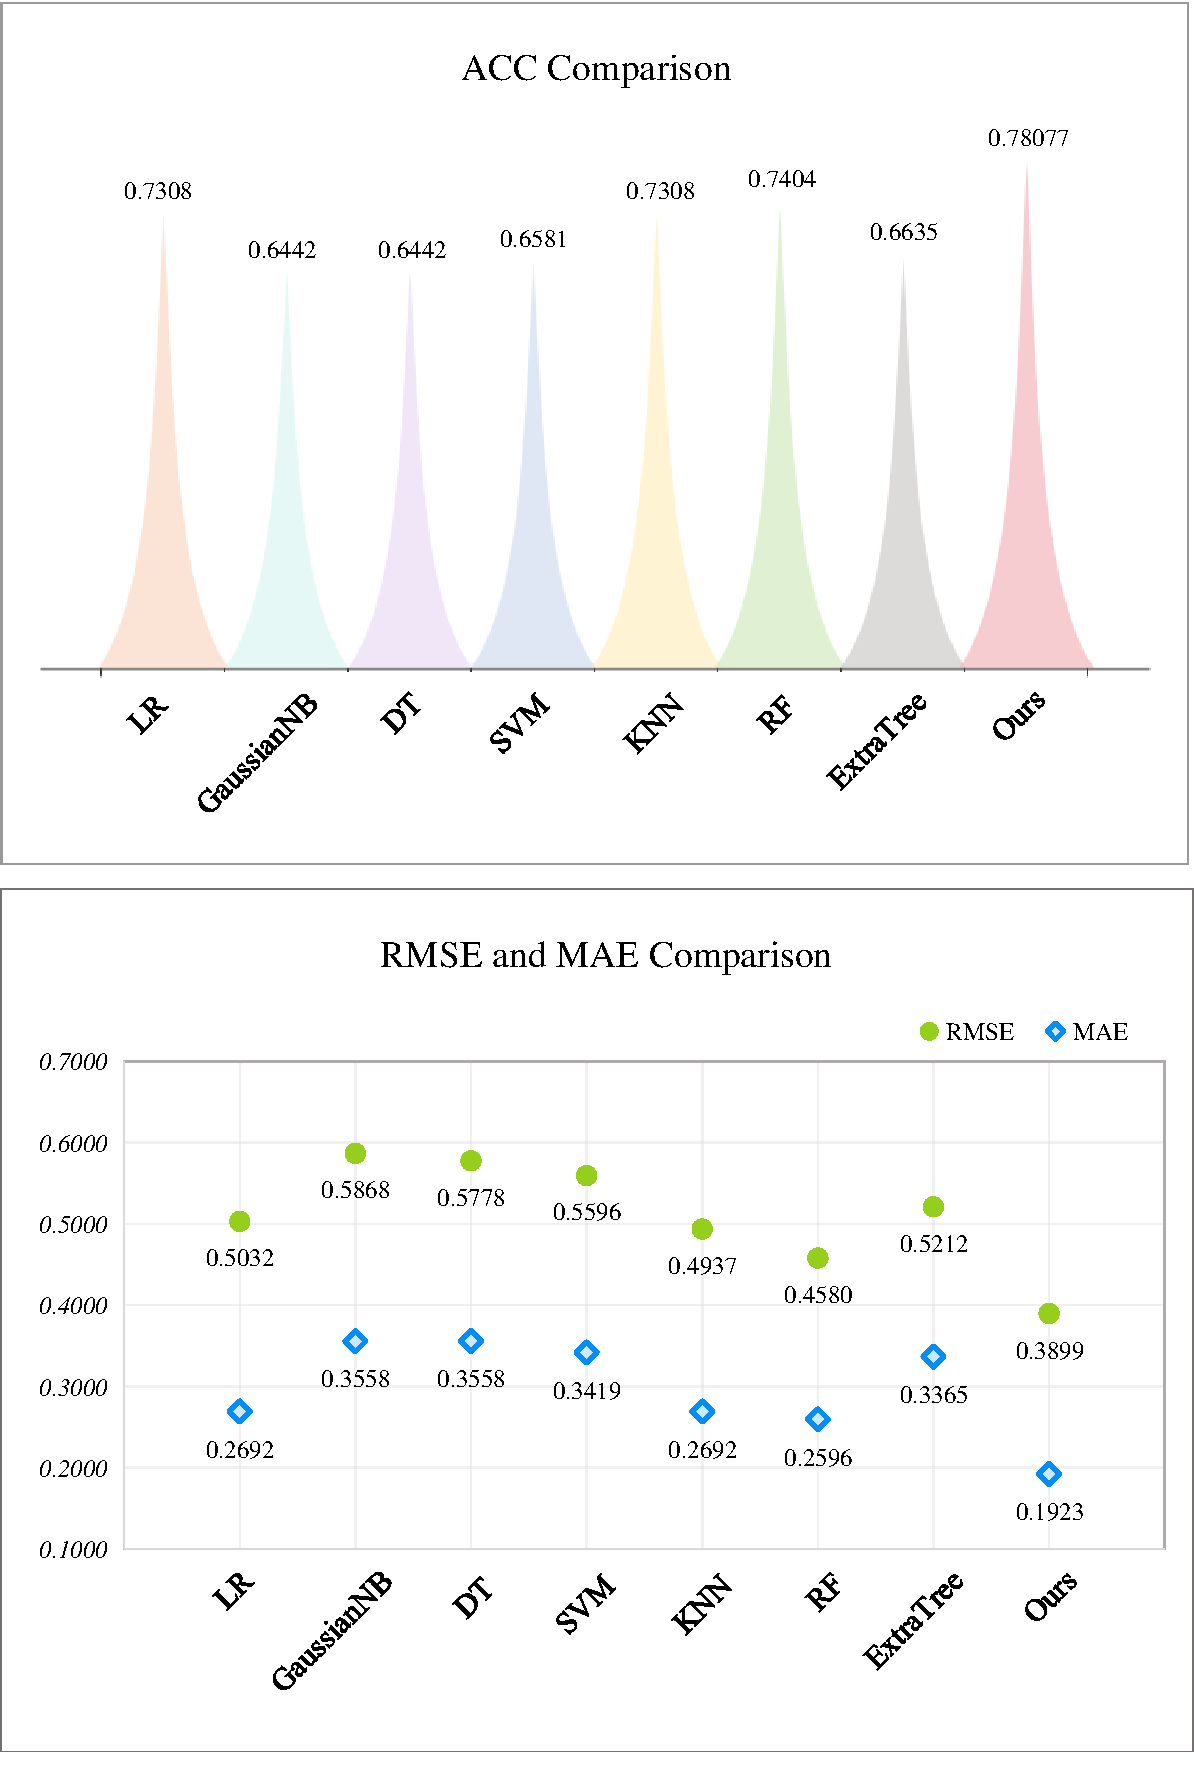
\includegraphics[width=0.7\linewidth]{figs/paper5accemsemae.pdf}
      \caption{采用不同ML技术的模型性能对比}\label{paper5accemsemae}
     \end{figure*}
\fi
     
    \begin{figure*}[ht]
      \centering
      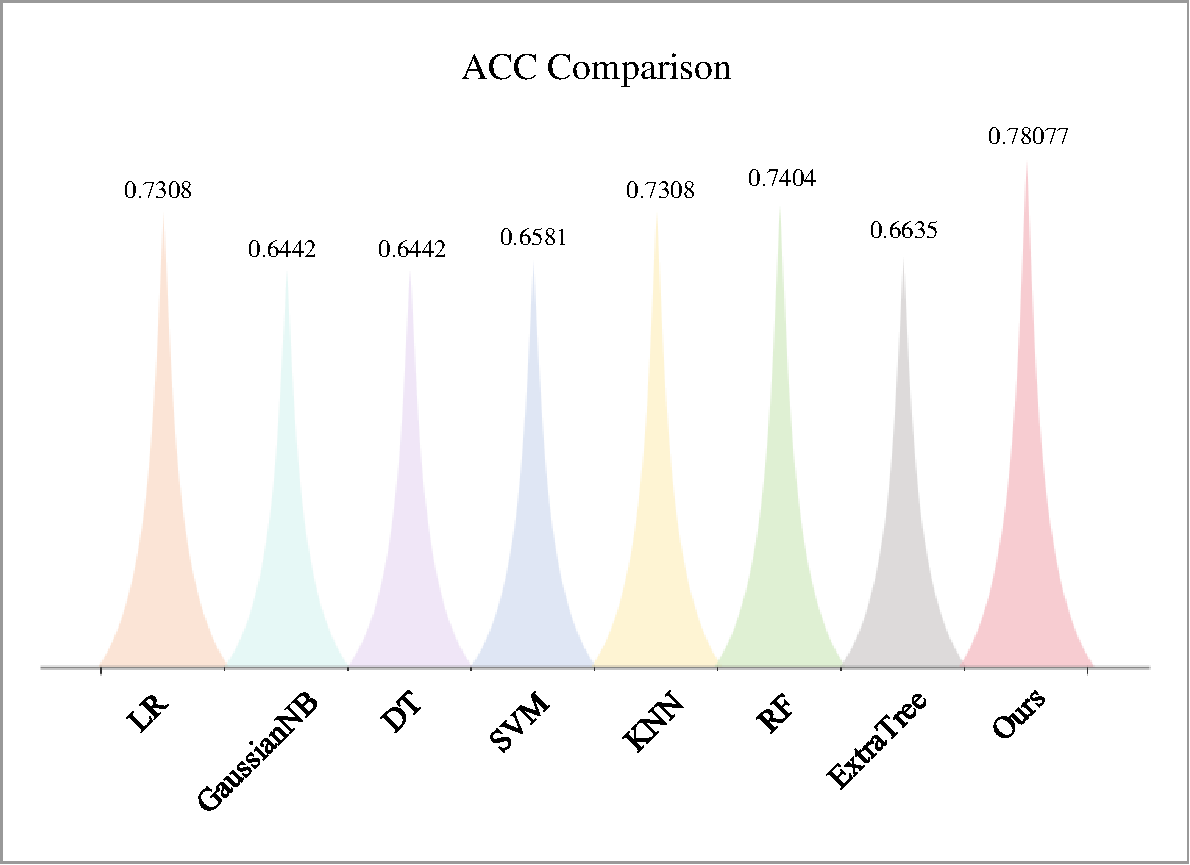
\includegraphics[width=0.85\linewidth]{figs/paper5accML.pdf}
      \caption{嵌入不同ML技术的模型ACC对比分析}\label{paper5accML}
     \end{figure*}

     
    \begin{figure*}[ht]
      \centering
      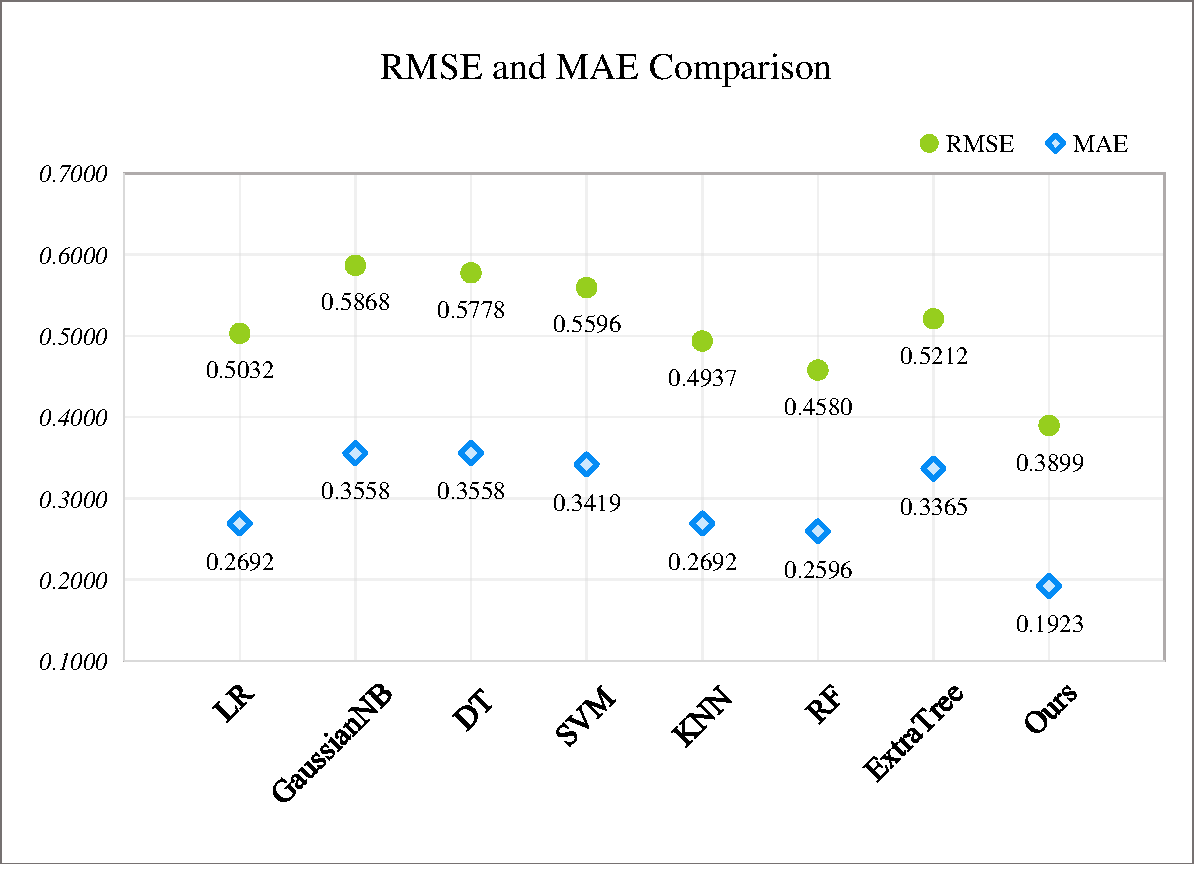
\includegraphics[width=0.85\linewidth]{figs/paper5rmsemaeML.pdf}
      \caption{嵌入不同ML技术的模型RMSE与MAE对比分析}\label{paper5rmsemaeML}
     \end{figure*}
     
\subsubsection{集成机器学习技术分析}
在本研究中,提出了一个集成了Adaboost算法的新模型。为了验证该模型的有效性,对其进行了一系列的性能测试,并将结果与其他几种流行的ML技术(支持向量机(SVM)、逻辑回归(LR)、高斯朴素贝叶斯(GaussianNB)、K最近邻(KNN)、决策树(DT)、随机森林(RF)、极端树(ExtraTree))进行了对比,如图~\ref{paper5accML}和图~\ref{paper5rmsemaeML}所示。本节采用了准确率(ACC)、均方根误差(RMSE)和平均绝对误差(MAE)这三个核心指标来衡量模型的预测能力。
ACC是衡量分类模型性能的常用标准,它反映了模型正确预测的样本占总样本数的比例。当准确率接近1时,表明模型具有极高的预测准确性。
RMSE则提供了预测值与实际值之间差异的量化度量。由于它是误差的平方根,因此对于较大的误差值,RMSE会更加敏感。一个较低的RMSE值意味着预测模型在数据拟合上更为精准。
MAE同样衡量预测值与实际值之间的差距,但与RMSE不同的是,MAE对所有误差值赋予相同的权重,因此它对异常值的影响较小。一个较低的MAE值通常指示着模型的预测误差较小,即模型性能较好。

\if 0
    \begin{figure*}[h]
      \centering
      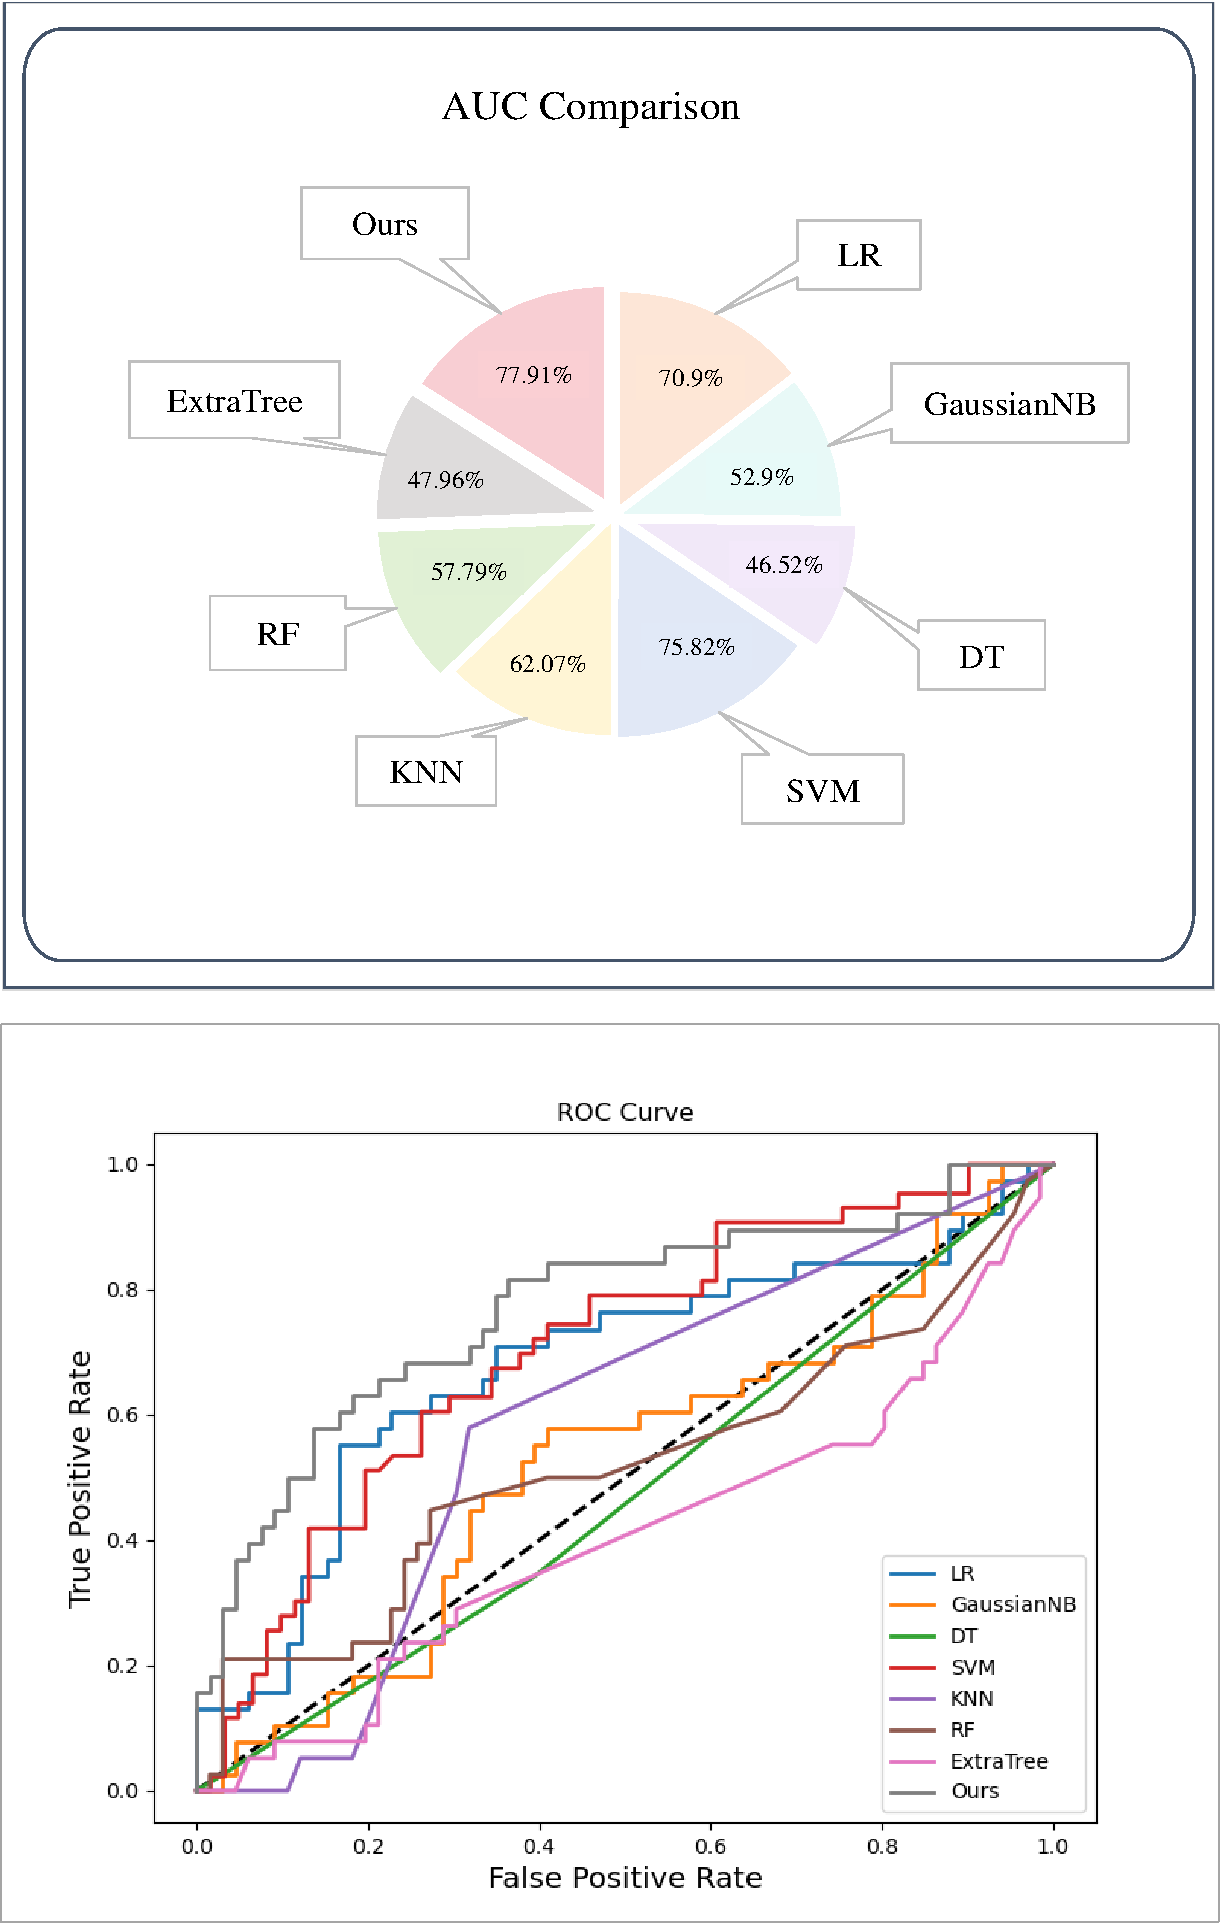
\includegraphics[width=0.7\linewidth]{figs/paper5aucroc.pdf}
      \caption{通过采用其他ML算法替代Adaboost的四项评价指标比较分析}\label{paper5aucroc}
     \end{figure*}
\fi
     
    \begin{figure*}[ht]
      \centering
      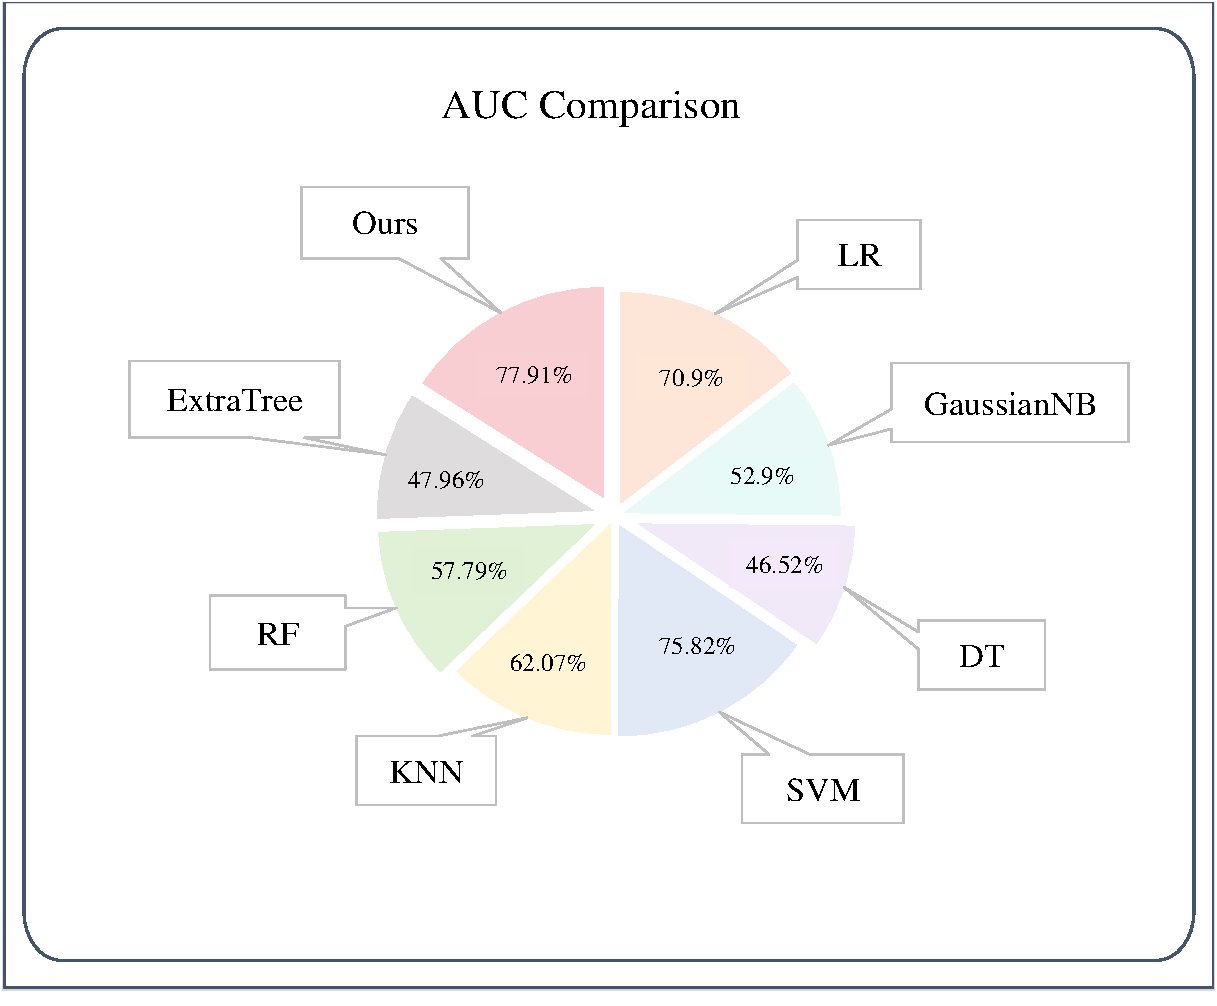
\includegraphics[width=0.85\linewidth]{figs/paper5aucML.pdf}
      \caption{嵌入不同ML技术的模型AUC对比分析}\label{paper5aucML}
     \end{figure*}
     
    \begin{figure*}[ht]
      \centering
      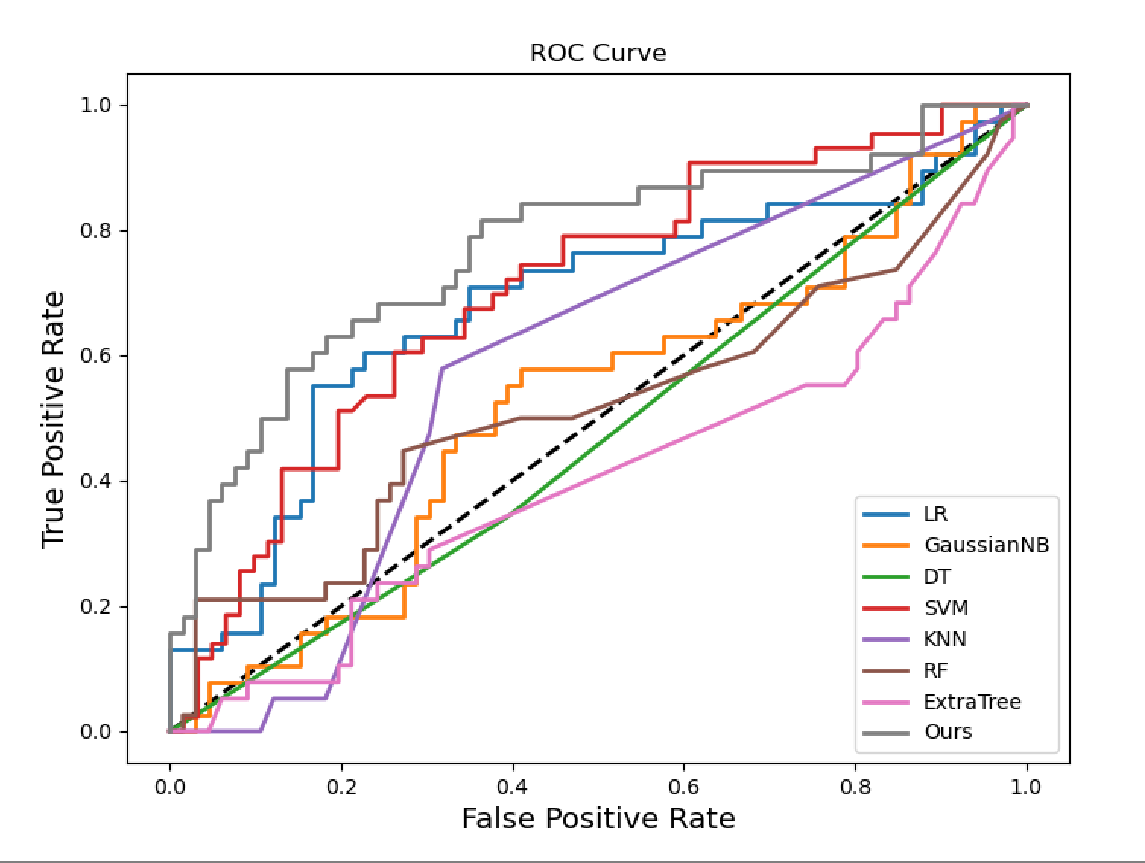
\includegraphics[width=0.95\linewidth]{figs/paper5rocML.pdf}
      \caption{嵌入不同ML技术的模型ROC对比分析}\label{paper5rocML}
     \end{figure*}

通过图~\ref{paper5accML}到图~\ref{paper5rocML}的直观展示,本节的方法在所有三个性能指标上都表现出色。特别是在ACC方面,本节的模型比其他算法表现得更为突出,比排名第二的随机森林算法(RF)高出了6.73个百分点。在RMSE和MAE的数值对比上,本节的模型也显示出了相对于RF算法分别低6.81\%和6.73\%的显著优势。
综上所述,本节的模型不仅在理论上设计精巧,而且在实际应用中也展现出了卓越的预测性能。这些结果充分证明了本节提出的方法在处理相关问题时的有效性和优越性。

\subsection{进展预测模型的探索与发现}  
弥散张量成像(DTI)作为一项先进的磁共振成像技术,已在近年来得到迅速发展。它利用多个不同强度的扩散敏感梯度,能够精确地描绘出人体内水分子的扩散能力及其移动方向,从而深入揭示生物组织,尤其是脑组织的微观结构特点。这种成像技术不需要对活体进行任何侵入性操作,便能直观地观察和分析白质纤维束的完整性和方向性,这对于研究神经系统的疾病具有重要意义。一些学者基于弥散张量成像(DTI)的研究探索了白质的变化,并发现与对照组相比,PD-MCI患者的额叶白质损伤更为显著,且与整体认知功能的损害以及多个认知领域的损害存在关联\cite{wang2020changes}。对于PD的复杂多样的神经机制,通过整合多种模态MRI特征,从多个层面和不同角度进行综合评估和分析,为进一步提高PD早期诊断和干预提供了潜在的生物标志物\cite{pyatigorskaya2018comparative,gu2016automatic,bowman2016multimodal}。Pyatigorskaya等人\cite{pyatigorskaya2018comparative}研究者结合了NMS-MRI中的黑质体积和信号强度特征以及DTI中的部分各向异性特征,成功地将PD诊断的准确率提升至93\%。Lei等人\cite{lei2018longitudinal,lei2017joint}开发的基于MRI和DTI的预测模型能够智能识别PD,并对临床评分进行准确预测,这在临床实践中具有重要的应用价值。Chougar等人\cite{chougar2021automated}则进一步探索了如何利用脑区(13个大脑区域)体积和DTI参数作为输入,并使用监督ML算法准确预测PD、PSP和MSA-P的分类。Shin等人\cite{shin2021cortical}的研究关注了MRI皮层厚度在预测PD患者从轻度认知障碍向痴呆转变中的作用。他们的研究结果显示,MRI皮层厚度能够有效预测个体的疾病进展,并且当与临床数据相结合时,其预测性能得到了进一步提升。这一发现强调了MRI技术在个体化医疗和精准治疗策略制定中的重要作用。

通过合并表 \ref{paper5singalAvg_AUC} 和表 \ref{paper5cmfDifferFeature_AUC} 中的数据,可以确定对PD预测贡献相对显著的临床指标,进而推断出与PD进展相关的潜在特征。这些关键的临床数据特征包括年龄、UPDRS第三部分分数、UPDRS总分以及UPSIT分数。

当前,可靠的网络表征技术的发展为在全脑连接层面理解神经疾病提供了新的途径。然而,目前关于使用白质数据来预测帕金森病(PD)进展的研究相对有限。Wee等人\cite{wee2011enriched}开发了一种基于网络的多变量分类算法,该算法利用白质纤维束数据,能够有效区分正常对照组和轻度认知障碍(MCI)患者。研究结果显示,这种分类框架能够为临床诊断以及与认知障碍相关的脑结构变化提供一种创新的替代和辅助手段。尽管如此,这项研究主要集中在阿尔茨海默病领域,对于PD的应用尚需进一步探索。


在本研究的预测模型中,除了纳入临床特征,还挑选了七个来自DTI变量的特征,这些特征涉及到脑白质的MD。研究发现,这些脑白质的特征在预测PD的发展进程方面具有重要作用,并且当与传统的临床特征相结合时,能够显著提升模型的预测准确性。
具体来说,仅依赖DTI全球白质特征构建的预测模型获得了0.44035的AUC值(方差为0.0185),而独立使用临床特征的模型AUC值稍高,为0.4414(方差为0.0187)。然而,当这两类特征被整合到同一个预测模型中时,模型的性能得到了显著的增强,AUC值跃升至0.7791(方差为0.1085),这表明DTI白质特征与临床特征之间存在着互补作用,共同为预测PD提供了更加丰富和精确的信息。


多模态融合技术通过整合来自不同来源和类型的数据,能够提供更为丰富和立体的信息,从而在理解复杂的生物医学问题时发挥着至关重要的作用。在PD的研究中,多模态融合尤其展现了其独特优势。例如,结合临床症状评估、扩散张量成像(Diffusion Tensor Imaging, DTI)和多巴胺转运体(Dopamine Transporter, DAT)显像等多种数据源,不仅能够揭示PD患者大脑结构和功能的细微变化,还能帮助医生更准确地评估病情的严重程度和进展速度。
图\ref{paper5ROCs_}所展示的五条ROC曲线直观地证明了多模态融合的有效性。在图\ref{paper5ROCs_}中,不同的颜色用于表示不同数据组合的预测结果。特别是在图(b)中,阴影区域展示了置信区间。分析结果指出,将临床数据与DTI或DAT影像数据结合使用的多模态方法,相较于单一数据源的预测方法,在预测帕金森病进展方面更为精确。尤其是将临床数据与DTI数据相结合的方法,展现出了最优的预测效果。单独使用某一种数据源的曲线(如临床数据、DTI数据或DAT数据)通常只能提供有限的信息,而一旦将这些数据结合起来,ROC曲线就会明显上升,表明模型的预测能力得到了显著提升。特别是当临床数据与DTI数据结合时,预测性能的提升尤为显著,这进一步验证了多模态融合在提高PD预测准确性方面的潜力。

\begin{table}[ht]
\centering
\caption{临床数据分别与DTI和DAT相结合进行预测}
\label{paper5twoClinDtiDat}
%\small
%\begin{tabular}{ccccc}
\begin{tabular}{p{2.3cm}<{\centering}p{2.2cm}<{\centering}p{2.2cm}<{\centering}p{2.2cm}<{\centering}p{2.2cm}<{\centering}}
\hline
\textit{Avg} & \textbf{AUC} & \textbf{ACC} & \textbf{SEN} & \textbf{SPE} \\ \hline
Clin-Dti           & \textbf{0.7791}       & \textbf{0.8077}       & \textbf{0.9464}       & \textbf{0.7470}       \\
Clin-Dat           & 0.6000       & 0.7385       & 0.8679       & 0.6298     \\ \hline
\textit{Vac} & \textbf{AUC} & \textbf{ACC} & \textbf{SEN} & \textbf{SPE} \\ \hline
Clin-Dti             &\textbf{0.1085}   & 0.1490       & 0.1417       & 0.1890       \\
Clin-Dat           & 0.1929    & \textbf{0.0923}      & \textbf{0.1041}       & \textbf{0.1516}     \\ \hline
\end{tabular}
\end{table}

正如表\ref{paper5singalAvg_AUC}、表\ref{paper5cmfDifferFeature_AUC}以及图\ref{paper5ROCs_}所展示的,将临床数据与DTI数据结合起来进行预测,其效果优于结合临床数据与DAT数据。此外,本节还进行了Mann-Whitney U检验,该检验进一步证实了临床数据与DTI数据结合预测的显著性,其结果在统计学上显著优于单独使用临床数据,p值达到了9.183e-4。这一结果强调了多模态数据融合在提高预测准确性方面的潜力。


  \begin{figure}[ht]
      \centering
      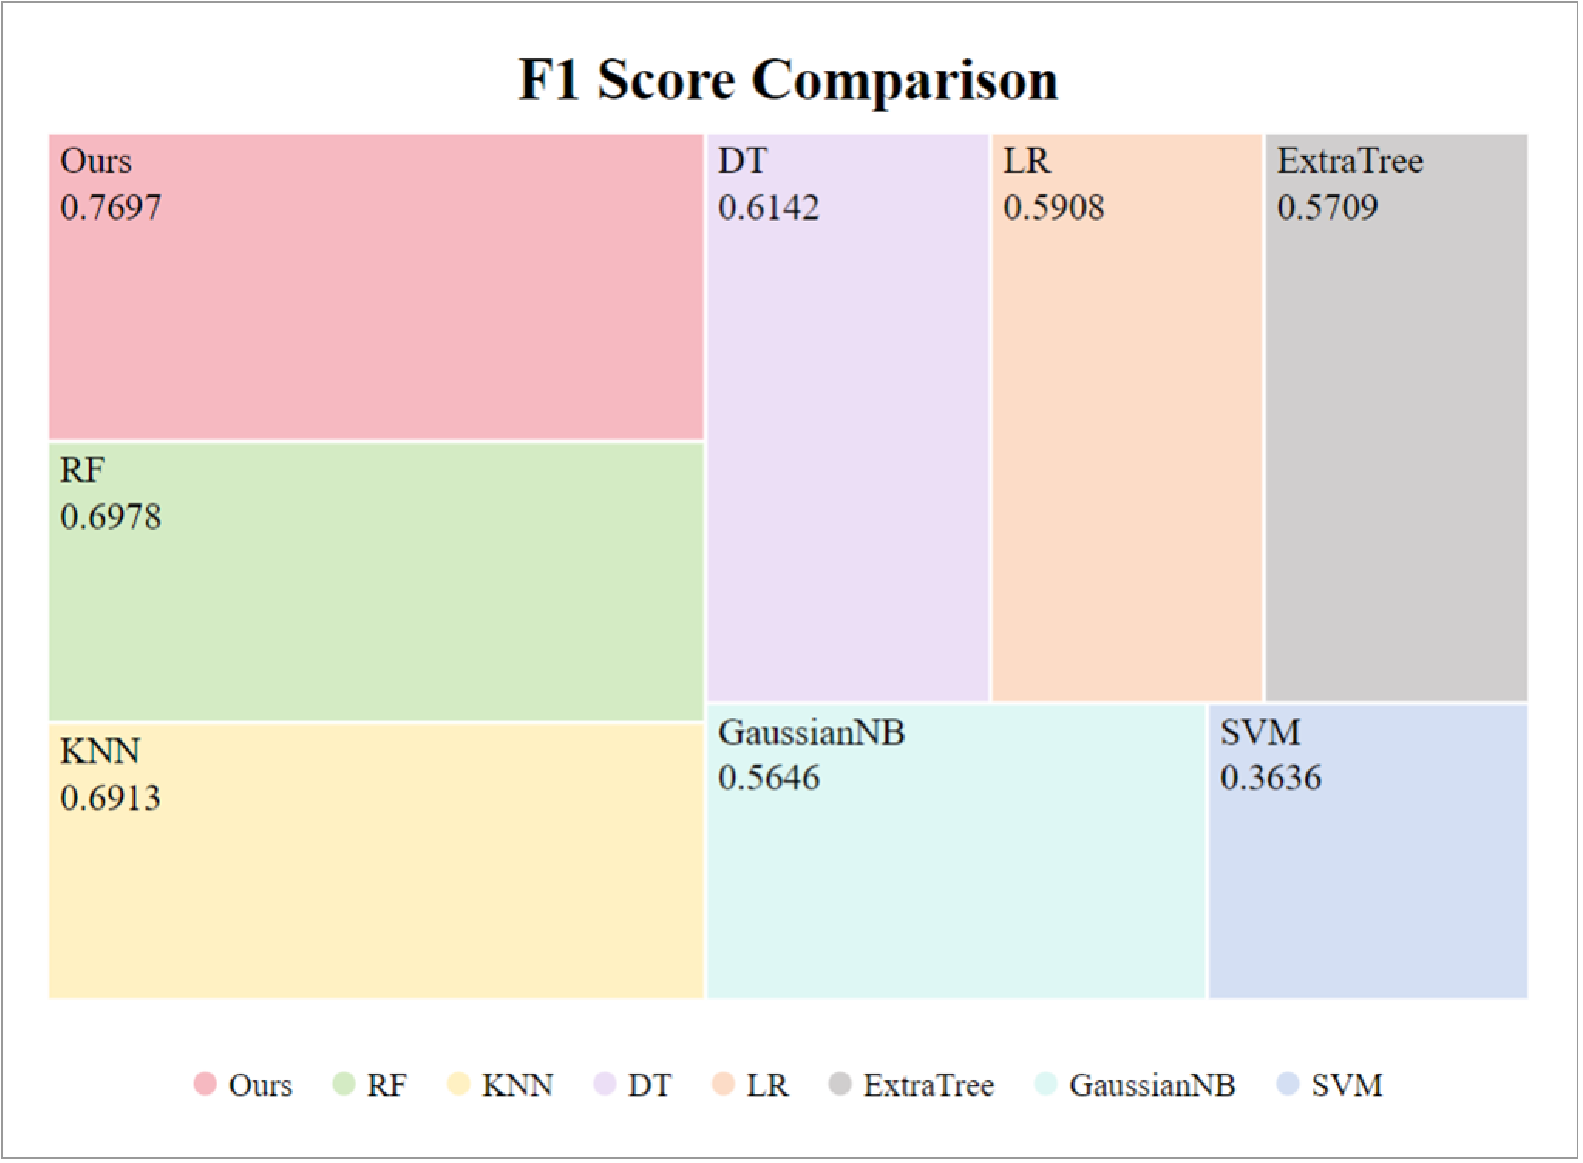
\includegraphics[width=0.85\linewidth]{figs/paper5F1_MLs2.pdf}
      \caption{嵌入不同ML技术的模型F1 score对比分析 }\label{paper5F1_MLs}
     \end{figure}

为了深入比较临床数据与DTI及DAT数据结合的预测效果,采用了ACC(准确率)、SEN(灵敏度)和SPE(特异性)这三项关键指标进行了详尽的分析,并将结果呈现于表\ref{paper5twoClinDtiDat}中。该表格所展示的数据是在经过8次测试后,各项指标的平均值(Avg)和方差值(Vac)。通过观察可以清晰地发现,在将临床数据与DTI数据相结合的情况下,无论是哪一项指标,其表现均显著优于其他组合,这一结果凸显了多模态融合在提高预测准确性方面的重要价值。

为了展现本节方法的卓越性,对不同机器学习算法替代情境下的AUC值进行了详细分析。AUC作为衡量模型分类能力的指标,其值从0至1不等,数值越大表明模型的性能越优。图\ref{paper5aucML}和图\ref{paper5rocML}可见,即使在AUC值上SVM算法排名第二,本节的方法仍领先SVM 2.09个百分点。

本节还计算了各模型的F1分数,并将结果呈现于图\ref{paper5F1_MLs}。从图中可以明显看出,本节的方法在F1分数上取得了最佳成绩,相比RF高出了7.19\%。虽然SVM在AUC指标上位居第二,但在F1分数方面却表现不佳。根据多维度的评估结果,本节的方法展现出了卓越的性能,证实了其在实际应用中的可靠性和稳定性。

综上所述,本节的研究发现将DTI的白质纤维束数据与临床特征相结合,能够显著提高对PD进展的预测能力。通过采用本文提出的CFMP方法构建的网络模型,不仅能够有效评估PD患者的疾病严重度,还能实时监控疾病的进展情况。这一突破性成果对于改进PD的早期诊断和治疗方案具有深远的影响,有望为患者提供更加精准和个性化的医疗服务,从而改善他们的生活质量。

\subsubsection{小结}
PD的发展是一个缓慢而持续的过程,其确诊通常依赖于临床表现和体征。随着疾病进入中期至晚期,治疗变得复杂且困难。因此,早期预测疾病进展对于实施及时有效的干预方案极为关键。但是,迄今为止还未发现精准的生物指标可以预判PD的病程发展,因此,构建一个能早期智能诊断该疾病的模型对于临床实践具有重大的意义。
DTI是一种能够量化大脑内水分子扩散性能的技术,它能够准确地衡量大脑中白质束的结构完好性,并且有助于识别早期病症的潜在迹象。本小节的研究采用基于纵向数据的研究方法,结合ML技术,整合早期PD患者的DTI数据和临床特征,构建了一个疾病进展预测模型。该模型有望为PD的早期诊断和治疗决策提供有力的影像组学支持。
该小节主要局限性在于仅利用了脑白质的平均扩散率(MD)指标进行分析,未能纳入其他相关指标,如分数各向异性(FA)和纤维密度(FN)等。此外,研究未从其他数据库获取数据来验证模型的泛化能力。在未来的研究中,将探索多模态融合分析,包括脑灰质结构数据、基因信息等,以期对PD及其他神经退行性疾病进行更深入的理解和研究。




\section{本章小结}
本章节主要对PD的预测展开了研究与分析,包括PD的静态与动态预测。其中,
在第\ref{chapter5.1:pdPredictReview}节中,回顾了基于ML的智能辅助帕金森疾病分类预测,强调ML技术的发展为帕金森病的智能诊断与健康测评提供了解决误诊或无法确诊的解决方案。通过对分类器训练的概述,强调了ML模型在挖掘大量数据中潜在规律方面的关键作用。
在第\ref{chapter5.2:pdCMF-Net}节中,提出了一种CMFP方法,基于跨模态数据融合的ML,用于智能辅助PD进展预测。该方法结合了DTI和临床特征数据,强调了PD疾病进展的漫长过程和对早期预测的需求。研究发现跨模态结合预测提高了单模态预测的准确性,DTI数据对临床预测性能的提升具有显著作用。
然而,本节的研究未涵盖神经科学机制,未来需要更深入地结合方法与神经科学,以提高准确性。